%%%namn p filien Raport felix andrad
%%% datum 2011 02 15
%%%%% mallen: nedladdad frn http://www.ee.iitb.ac.in/~trivedi/LatexHelp/latexsample.htm


%% This LaTeX-file was created by <guest> Sun Jan  3 14:45:46 1999
%% LyX 0.12 (C) 1995-1998 by Matthias Ettrich and the LyX Team

%% Do not edit this file unless you know what you are doing.

%%%%%%%%%%%%%%%%%%%%%%%%%%%%%%vikitga ting start
\documentclass[10pt]{report}
%%%%%%%%%%%%%%\documentclass[12pt]{article}
\usepackage[T1]{fontenc}
\usepackage{geometry}
\geometry{verbose,a4paper,tmargin=15mm,bmargin=30mm,lmargin=30mm,rmargin=20mm}
\usepackage{graphics}
\usepackage{setspace}


%%%%%%%%%%%%%%%%%felix inlagg
\usepackage[applemac]{inputenc} %% latin1 or applemac
\usepackage{wrapfig}
%\usepackage[utf8]{inputenc}
\usepackage[swedish,english]{babel}
\usepackage{amsmath}
%\usepackage[retainorgcmds]{IEEtrantools}
\usepackage[gs]{graphicx}
%%%%%%%%%%%%%%%%%felix inlagg

\usepackage{colortbl}
\usepackage{multirow,bigdelim}


\setcounter{secnumdepth}{5}
\setcounter{tocdepth}{5}
\onehalfspacing

\makeatletter


%%%%%%%%%%%%%%%%% LyX specific LaTeX commands.
\newcommand{\LyX}{L\kern-.1667em\lower.25em\hbox{Y}\kern-.125emX\spacefactor1000}
\makeatother
\renewcommand\bibname{References}
%%%%%%%%%%%%%%%%%%%%%%%%%%%%%%




\begin{document}
%\bibliographystyle{plain}


%%%%%%%%%%%%%%%%%%%%%%%%%%%%%%frsta sidan
\begin{titlepage}
\thispagestyle{empty}
\vspace*{0.7cm}
{\centering	 
\large

\includegraphics[width=4cm]{__meta_doc/kth_rgb.jpg}\\[-1mm]
\vspace{1.5 cm}
{\Large\bf A Heuristic Approach to the Multiagent Pursuit and Evasion Problem in a Polygonal Enviroment.}\\
\vspace{1.5cm}
\bf{Bachelor Thesis}\\
\vspace{.5cm}
\it
by \\
\vspace{.25cm}
\rm
\selectlanguage{swedish}
{\large \bf {Felix Blumenberg}}\\
{\large \bf {felixb@kth.se}}\\
{\large \bf {Fredrik B�berg}}\\
{\large \bf {fbaberg@kth.se}}\\
{\large \bf {Mats Malmberg}}\\
{\large \bf {matsmalm@kth.se}}\\
\selectlanguage{english}
\vspace{1cm}
{\it{under the guidance of}} \\
\vspace{.5cm}

\hspace{.05cm} {\large \bf {Doctoral Student Johan Thunberg}}\\
\hspace{.05cm} and\\
\hspace{.05cm} {\large \bf {Professor, Ph.D. Xiaoming Hu}}\\
\vspace {0.75cm}
%\iitbseal\ \\

%\begin{figure}[h]
%\hspace{6cm}
%\vspace{5cm}
%{\centering {\includegraphics{iitlogo1.ps}}\par} LOGO!
%\end{figure}

Department of mathematics\\
Division of Optimization \& Systems Theory \\
Royal Institute of Technology KTH, Sweden\\
{\centering
\hspace{6.5cm}Apr 2011}
}
\pagebreak
\end{titlepage}
%%%%%%%%%%%%%%%%%%%%%%%%%%%%%%



%%%%%%%%%%%%%%% %%%%%%%%%%%%%%% tv abstrakt olika sprk olika sidor
\selectlanguage{english}
\vspace{2in}
\begin{abstract}
In this paper heursitic algorithms are developed for the pursuit evasion problem in polygonal enviroments. In this problem, continuous trajectories shall be constructed for a group of pursuers, searching for an evader, in such a way that the evader is guaranteed to be seen at some time during the search.
%The problem consists of constructing continous trajectories for a group of pursuers, searching for an evader, in such a way that the evader is guaranteed to be seen at some time during the search.
Three fundamentaly different heuristic methods are considered: tabu search, genetic algorithms and greedy methods. The result is three heuristic algorithms. Two algorithms are readily implemented and fast yielding solutions of high quality compared to previous work to the best of our knowledge. The report attains and evaluates statistics on runtime, and the quality of the solution for a vast amount of randomly generated enviroments.\\
\\Keywords: Heuristic algorithms, tabu search, greedy methods, genetic algorithms, pursuit and evasion.
\end{abstract} 

\selectlanguage{swedish}
\vspace{2in}
\begin{abstract}
Abstract p� SVENSKA
\end{abstract} 

\selectlanguage{english}
%%%%%%%%%%%%%%%%%%%%%%%%%%%%%%


%%%%%%%%%%%%%%%%%%%%%%%%%%%%%%% innehllsfrteckning
\pagenumbering{roman}
\tableofcontents{}

%%%%%%%%%%%%%%%%%%%%%%%%%%%%%%%
\listoffigures
\newpage
\newenvironment{mydef}[1]{\begin{definition} #1 \mbox{\\}
\rm}{\end{definition}}
%%%%%%%%%%%%%%%%%%%%%%%%%%%%%%%


%%%%%%%%%%%%%%%%%%%%%%%%%%%%%% arbetet
\pagenumbering{arabic}

%%%% 	vill du lgga  in ngot dokument ngon stans lgg det i rtt ordning nedan
%%%%     samt anvnd nedstende document som mall nr du skirver

\chapter{Introduction}

\section{Objective}
The aim of this report is to construct heuristic algorithms that solve the pursuit and evasion problem in two dimensional polygonal environments. The original pursuit and evasion problem is fully formulated in chapter two. Informally it can be formulated as ``given an environment with static obstacles, and a specific number of pursuers, construct a search strategy for the group of pursuers such that the evader is guaranteed to be seen''. In \cite{paper3} a framework is presented for solving the problem. In this framework a method is provided for finding the optimal solution. In practice this algorithm is not very applicable though, since even for small areas the computational time is large. This motivates the introduction of heuristic methods. By sacrificing optimality, our aim is to use heuristic methods to find sufficiently good solutions within a reasonable computational time. These methods have, to the best of the authors' knowledge not been used in this context before.
%%
\section{Background}
\subsection{What is optimization?}
The aim of optimization is to find the best available value of an objective function, given a defined domain. % Refer to other literature?
The mathematical theory of optimization offers a variety of methods to solve a wide range of problems. To approach these problems and find a solution, it is important to identify the characteristics of the problem considered. Relevant distinctions can be made by studying the problem's complexity. Complexity is strongly related to the computational time. There are many different complexity classes of problems, but two of the most fundamental are the P and NP.

subsection{P \& NP problems.}
%skriva om hela sektionen??
The distinction between these two reveals the difficulty of our problem. This will only be a brief description, for a more detailed and interesting description please see \cite{NP}.\\
Informaly one can say that P are problems that are easy, and NP are problems that are difficult. In NP ther is a subcalss called NP-complete.\\
NP-complete are the hardest problems in NP\cite{adk19}. Such a problem is NP-hard and in NP.
NP-hard are problems that are At least as hard as the hardest problems in NP. But such problems need not be in NP\cite{adk19}.\\
Related work has stated that the problem studied in this report are in fact of the class NP-hard \cite{paper1}.\\ % Is it paper one?
The conscvens of the problem beeing NP-hard is that one can not construct analytick algorithems that provieds an optimal solution in a resnabul amount of time.


\subsection{P \& NP problems.}
%skriva om hela sektionen??
The distinction between these two reveals the difficulty of our problem. This will only be a brief description, for a more detailed and interesting description please see \cite{NP}.

P is the set of problems which can be solved by a deterministic Turing machine using a polynomial amount of computation time.
Cobham Edmonds thesis holds that P is the class of computational problems which are "efficiently solvable" or "tractable". In practice, some problems not known to be in P have practical solutions, and some that are in P do not, but this is a useful rule of thumb.

NP refers to Non-deterministic Polynomial time, and can be intuitively described as the set of problems for which, a found solution can be verified to actually be the correct solution, using a deterministic Turing machine using a polynomial amount of computation time.

A set of descriptions that leads one to wonder whether
\begin{equation}
P = NP
\end{equation}

In what the essence is:
Suppose that solutions to a problem can be verified quickly. Then, can the solutions themselves also be computed quickly?
Or stated differently, does it exist such an algorithm that can calculate such a solution quickly?
An unsolved question considered by many to be the most important problem in the field of computer science.

Within the class NP there are a few subclasses one of them are called NP-hard 
Related work has stated that the problem studied in this report are in fact of the class NP-hard \cite{paper1}, % Is it paper one?
and hence the chances of finding an algorithm that produces an optimal solution in polynomial time are greatly reduced. As stated above it is still an open question whether such algorithms actually exist for NP problems.
%%
\subsection{A near optimal solution.}
As mentioned in \cite{paper1} the problem under consideration is at least NP-complete. The consequences of this is that the chances of finding an optimal solution within reasonable computional time are seen to be very low. Thus we are imposed to sacrifice optimality, in order to gain computational efficiency. This sacrifice opens a large spectrum of possible approaches to the problem.
%%
\subsection{Heuristic methods}
Heuristic methods is a branch of methods used in computer science and mathematics. According to \cite{heuristics}``A heuristic search method can be seen [35] as a procedure taking advantage of the problem structure in order to identify a good solution within a reasonable amount of computing time.''
In general, heuristic methods does not provide optimal solutions.% Reference?



Though sometimes, for specific situations, it can be proven that a certain heuristic algorithm's solutions are optimal. Also, there is no general way of proving whether a heuristic algorithm provides an optimal solution. Despite this fact heuristic methods often provide extremely efficient and relevant algorithms. Very often they reduce the computational time needed for a solution greatly. There are even several occasions where a heuristic method is prefered to an analytic method. A few examples are:
\begin{itemize}
\item When there is no known algorithm for solving a specific problem, a heuristic is the only way to approach a solution.
\item A algorithm can sometimes be difficult to implement. Heuristics can sometimes be used instead because they are easy to implement and known to produce good results.
\item When the problem is too difficult to solve efficiently and quickly with analytical methods. A heuristic method could overcome that and give an acceptable but probably not optimal solution.
\end{itemize}

The last point corresponds to the problem we are dealing with.
\section{Outline}
\chapter{Problem formulation}
%%describe feasible environment? referenced to from chapter 3

This paper is an extension of the paper ``A Boolean Control Network Approach to Pursuit Evasion Problems in Polygonal Environments''\cite{paper1}. Our main purpose is to use three conceptually different heuristic methods to try to construct algorithms that efficiently solves the problem stated in the section below. We will also try to implement these algorithms in ANSI C to evaluate the quality and efficiency of the algorithms. The efficiency is quantified as the runtime needed for the algorithm to construct a solution. The quality of the solution is quantified in terms of path length. We will also discuss how the efficiency and quality of the solutions depend on the size of the environment and the number of pursuers.
\section {The Pursuit \& evasion problem with multiple pursuers.}
Following the previous work of Johan Thunberg  et. al.\cite{paper1}, the pursuers and the evader are modelled as points moving in the polygonal free space, F . Let  $e(\tau )$ denote the position of the evader at time $\tau \geq 0$. It is assumed that $e : \lbrack 0, \infty) \to F$ is continuous, and that the evader is able to move arbitrarily fast. The initial position e(0) and path e is not known to the pursuers. At each time instant, F is partitioned into two subsets, the cleared and the contaminated, where the latter might contain the evader and the former might not. Given N pursuers, let $p_i (\tau ) : \lbrack 0, \infty) \to F$ denote the position of the i:th pursuer, and $P = \lbrace p_1 , . . . , p_N \rbrace$ be the motion strategy of the whole group of pursuers. Let V (q) denote the set of all points that are visible from $q \subset F$ , i.e., the line segment joining q and any point in V (q) is contained in F .\\
\\
\textbf{The original Problem (Pursuit Evasion).} \emph{ Given an evader, a set of N pursuers and a polygonal free space F , �nd a solution strategy P such that for every continuous function $e : \lbrack 0, \infty) \to F$ there exists a time $\tau$ and an i such that $e(\tau ) \subset V (p_i (\tau ))$, i.e., the pursuer will always be seen by some evader, regardless of its path. }

\section{Discretized problem}
Notations from \cite{paper1} is used.
\begin{description}
\item[Tile]A tile is...
\item[Feasible solution]A feasible solution is...
\item[Complete solution]A complete solution...
\item[Incomplete solution]A incomplete solution...
\item[Path]A path is...
\item[Secured]A secured...
\item[Area]An area is...
\item[Pursuer]A pursuer...
\end{description}
\section{The problem formulation of this paper}
Given the original pursuit \& evasion problem presented in the previous chapter, section 1.4.4. Our aim is to:
\begin{enumerate}
\item[-] Construct three heuristic algorithms that solve the problem.
\item[-] Implement the algorithms and evaluate their efficiency and the quality of the solutions presented.
\item[-] Collect data from the results of implemented algorithms' and discuss whether any new conclusions can be made on how to approach the original problem.
\end{enumerate}

\section{Approach}
The work will be divided into six sequentially performed subtasks, each will be discussed in more detail below. The subtasks are:
\begin{enumerate}
\item[-] Find three relevant heuristic methods for our problem and do an in-depth research on them.
\item[-] With the chosen heuristic methods, construct three algorithms that solves the given problem.
\item[-] Create an simulation environment for the algorithms.
\item[-] Implement the algorithms.
\item[-] Run the algorithms to collect adequate data.
\item[-] Evaluate the data and draw conclusions.
\end{enumerate}

As mentioned in Chapter 1, Section 1.4.5. there are a vast amount of different heuristics. In this report we decided to use the heuristic concepts from greedy methods, tabu search and genetic programming to construct the algorithms. Greedy methods are local and deterministic in their approach. Both tabu search and genetic algorithms are stochastic and global in their approach, but they differ significantly in how they examine and construct feasible solutions. We have intentionally chosen our methods so that each method strongly differs in its characteristics from the other two. The reason for this decision was that we wanted to see if some conclusion could be made about if any specific characteristics would be favourable for solving our problem.\\
\\
The subtask to construct the algorithms is self-explanatory in what it means. More information about the process is given in chapter four.\\
\\
Since the problem is NP-hard and the algorithms are heuristic the need for a simulation environment is obvious. All implementations are made in ANSI C \cite{C-bok}, due to computational efficiency. The requirements on the simulation environment is that it should be possible to construct random feasible environments of specified size for the problem, run all algorithms on the environment and print the results into a file. A more in-depth description of how the simulation environment is implemented can be read in chapter three.\\
\\
The subtask of implementing the algorithms is also self explanatory in what it means. More information about the implementation of the algorithms is found in chapter four.\\
\\
Once all the implementations are done, simulations will be executed to collect data. The output data from the algorithm is runtime and solution paths for the pursuers. Also the environments' size, density and number of pursuers is known for each execution. The results are presented and discussed in chapter five and six.
\chapter{Simulation Environment}
%The chapter gives a description of the simulation environment we have created. Presenting how we created it, why we needed to create it and motivation of the choices made. First we give an short overview of the parts that are in the enviroment, and a definition of in/out data. Motivating all our choices made concerning limitations in the enviroment, and also describing positive features of our enviroment.\\
In order to attain the data needed for a comparison of our different algorithms it was nessecary to construct a good testing environment. We decided to create this environment by the use of two separate parts. One part is called the "Map generator". This part creates a map of the environment, tests the feasibility and prints feasible environments into an output file. The other part is called the "Network generator". This part reads an environment from a file, creates a graph network to the corresponding map and gives each node in the network its relevant information.\\
\section{Map generator}
The Map Generator (MG) creates random feasible environments. A feasible environment is described more in detail in section 2, but in short one could say that an environment is feasible if it is simply connected and can be divided into a finite set of convex regions. Given the desired size and the density (percentage of obstacles per total area) as inputs, the MG creates square shaped feasible environment with randomly placed obstacles and saves the map in an external file. For simplicity we have chosen to construct environments consisting only of square regions. We suggest that this does not result in a loss of generality since any feasible environment can be approximated arbitrarily good by a sufficiently fine meshing of squares. \\
\\We will now show in a more detailed manner how the MG works. First we present some pseudo code describing the algorithm and then some in depth comments to the code.\\
\\\noindent\emph{Pseudo-code, Map Generator:}
\begin{verbatim}
1  input variables:
2  Size;  // Specifies the width and height of the square matrix  A.
3  NumberOfEnv; // Specifies how many feasible environments to create.
4  Obstacle; //  Specifies the number of obstacles in percents, e.g. 
number of obstacles per total area of A.
5  while ( i < NumberOfEnv ){
6  	A = CreateMatrix( Size); 
7  	PlaceObstacle( A, Obstacle);
8  	if (Test( A)=TRUE){ 
9 		fprintf( fileOK, "\n \n");
10 		i++;
11	}else{
12 		fprintf{file NotOk, "Does not work: \n");
13 	}
14 }
\end{verbatim}
We will now describe the steps and the functions in the pseudo code above in more detail:
\begin{itemize}
\item First we introduce the needed variables to define how many and what kind of environments to create. 
\item The algorithm starts off by entering a while loop running until the loops content has created the desired amount of feasible environments. 
\item The function CreateMatrix(int arg) creates an matrix of dimensions $(arg \times arg)$ with every element equal to one. In our map a one corresponds to a feasible square region for the pursuer or evader to thread. 
\item Next we call the function PlaceObstacle(int A, int Obstacle). This function takes the input matrix A and using a randomizing function rand() places zeros in the matrix. The zeros corresponds to obstacles, e.g. squares that can't be seen through and can't med treaded.
\item The function Test (int A) tests if all the tiles in the given matrix A can be connected. If A is connected the environment is feasible and the function returns TRUE, if not it returns FALSE. First Test() finds the first element in A equal to one, starting from the upper left corner going to the right. Then it performs a breadth first algorithm to test if all tiles can be found from the starting point. If so, the enviroment is connected, and thus feasible.
%When such element has been found its index is pushed on a stack. Next we enter a loop that runs for as long as the stack is not empty. First it pops an index from the stack and checks if this index has been accounted for (e.g. if it lies within a vector C). If not accounted for, all the neighbor elements that are equal to one has their index pushed on the stack. Lastly the poped index is put into C, since it has been accounted for. The algorithm starts over by poping a new index and rerunning the loop. 
\end{itemize}
\section{Network generator}
The Network Generator (NG) generates a node network from an environment matrix. Each node contains data of its adjacent nodes, all the nodes visible from it and its current state. The input to NG is an environment matrix.\\
\\
\noindent \emph{Pseudo-code, Network Generator:}
\begin{verbatim}
1. A = environmentFromFile();
2. Node B = createNodeMatrix();
3. for(Node N in B):
    3.1. setName(); // Set name to the row and column for N in B.
    3.2. setMove();
    3.3. setVision();
\end{verbatim}
We will now describe the steps and the functions in the pseudo code above in more detail:
\begin{itemize}
\item environmentFromFile() sets A to an environment matrix, consisting of zeros and ones, which is read from an input file. The matrix in the file could either be generated by the MG or constructed by hand.
\item A Node is a datastructure that contains a name, pointers to all adjacent Nodes and pointers to all Nodes that can be seen by the actual Node.
\item createNodeMatrix() sets B to a matrix of the same dimensions as A, where each element is of the datatype Node.
\item setMove() creates pointers from the current node N to all feasible vertically and horizontally adjacent nodes.
\item setVision() creates a list of pointers to all visible nodes in B from the current node N. A node B is visible to N if both B and N can be contained inside a rectangle that does not contain non-feasible region.
%\begin{description}
%  \item[First] \hfill \\
%  The first item
%  \item[Second] \hfill \\
%  The second item
%  \item[Third] \hfill \\
%  The third etc \ldots
%\end{description}

%Visible Nodes is each node that can be connected to N by a straight line without passing through a non-feasible Node. The visible nodes are decided by first calculating Umax and Dmax which is the number of columns between N and the first non-feasible Node upwards and downwards in the same row, and Lmax and Rmax which is the number of rows between N and the first non-feasible Node in the same column as N. Each Node up to Lmax columns to the left of N and Rmax columns to the right of N is visible. For each of these Nodes every Node that is feasible and in the same column, at most Umax rows above or the first non-feasible Node, whichever comes first, and at most Dmax rows below or the first non-feasible Node, is visible. Umax and Dmax is re-calculated for every column to the left and to the right of N, and is the minimum of the number of the current Nodes Umax and Umax for the previous Node in the same row, with the same applying for Dmax.
\end{itemize}
\chapter{Methods}
In this report it was decided to use the heuristic concepts from greedy methods, tabu search and genetic algorithms to construct the algorithms. These methods has been intentionally chosen so that each method strongly differs in its characteristics from the other two. Greedy methods are local and deterministic in their approach. Both tabu search and genetic algorithms are stochastic and global in their approach, but they differ significantly in how they examine and construct \emph{feasible solutions}. The reason for this decision was to examine if some conclusion could be made about if any specific characteristics would be favourable for solving our problem. 

\pagebreak
\section{The genetic algorithm approach}
Genetic algorithms are based on the idea of evolution, that the most suited individuals tend to live longer and reproduce. 
\subsection{Description of genetic algorithm}
In Genetic Algorithms, or GAs, a population is simulated in an artificial world using a combination of reproduction, gene crossover and mutation, with a given goal for the population to achieve.
\\
Due to the need to simulate the population and evaluate individuals, often multiple times, GAs are not well suited for all kind of problems. When there exists an analytical solution it may be better to use that. However, if the problem can be simulated, both problems without analytical solutions and problem with complicated analytical solutions can be handled by GAs, although it is never guaranteed to give an optimal solution.\\
\\
As in nature, a population consisting of individuals are used. As a simplification, each individual has one chromosome, containing one or more genes. During each generation, individuals are selected and paired for reproduction, and their genes are combined to form new children.\\
\\
%% Generational / Steady-state
GAs can either be steady-state or generational, where steady-state means that the current population is altered, and generational is when a new generation is created and replaces the old.\\
\\
A GA can be described by the following steps:
\begin{enumerate}
\item Initial population
\item Repeat:
\subitem Evaluation
\subitem Breeding
\subsubitem Selection
\subsubitem Crossing
\subsubitem Mutation
\subsubitem Replacement
\subitem Search Termination
\end{enumerate}
%% Fitness function
To be able to compare different individuals, a fitness function is used. The fitness function should calculate a score for an individual, depending on how fit the individual is in relation to the goal.

%% Breeding
To make sure that evolution is performed, a breeding step is used, during which two individuals are selected and used to create two new individuals. The creation is done first by crossover and then by mutation.\\
%% Selection (parents)
There are different procedures that can be used for each step of the algorithm, for selection five different methods are Fitness Proportionate Selection, Random Selection, Fit-Fit, Fit-Weak and Elite selection.\\
In Fitness Proportionate Selection, of which Roulette Selection is one example, the probability of choosing a more fit individual is higher than to select a less fit individual.\\
In Random Selection, the probability to be selected is equal for all individuals. \\
With Fit-fit, the two most fit individuals are selected, and thereafter the two next most fit are selected.\\
With Fit-Weak, the most fit and the least fit individual are selected.\\
In Elite selection the best individual is chosen. This selection procedure should be used in combination with another selection method.\\
\\
%% Crossover
For Crossover there are different methods, a few of those are n-point shuffle crossover, uniform crossover and variable crossover.\\
\\
%% Mutation
\\Mutation is important in GAs since it makes sure that all the search space can be reached, even if the initial population did not cover all of it. It can be implemented as 'bit-flip', if the gene is binary encoded, where a 0 is changed to 1 and 1 to 0.\\
\\
%% Replacement
When breeding has been completed, in order to not increase the population size, a replacement has to be performed. For this there are several methods, such as Weak Parent, Both Parents, Weakest Individual and Random.\\
In Weak Parent, a weaker parent is replaced by a stronger child.\\
In Both Parents, the children replaces the parents.\\
In Weakest Individual, the children replaces the two weakest individuals in the population, if the children are fitter.\\
In Random, the children replaces random individuals in the population.\\
\\
%% Termination
To make sure the algorithm ends at some point, a termination condition has to be used. It can be a maximum number of generations, a limit in fitness sum, a median fitness, best individual or worst individual.\\
With Fitness sum, the algorithm will terminate when the sum of the fitness for the population is less than or equal to a specified value.\\
With Median fitness, a range for the fitness is specified.\\
With best individual, the algorithm will terminate when the minimum fitness drops below a convergence value and thereby guarantee at least one good solution while saving time.\\
With Worst Individual, the algorithm will terminate when all individuals in the population has a fitness value lower than the convergence value.\\
%%%% Development process of the genetic algorithm
\subsection{Development process of the genetic algorithm}
The first idea to use  was to use an existing framework for Genetic Algorithms, such as LibGA or GAUL, to save time on programming. Due to the implementation of the libraries, for this application it was determined to be faster to write a new implementation.\\
%% Random
\\After reading the parts of the source code of the existing libraries and Johan Thunberg's Boolean Control software, for ideas, a first attempt to a program was written. The first version was a boolean control network, where feasible solutions were generated by using a random function to generate numbers between 0 and 4 to indicate if the pursuer were to move left, right, up, down or stand still.\\
%% Encoding
\\To encode the genes, an integer based encoding was used. According to literature \cite{GAHandbook1}, binary encoding is faster, but as this is an attempt to implement heuristic methods and an integer encoding is easier to debug, it was used instead. Each integer in the gene is called an allele.\\
%% Generational
\\Generational GA was used, because of easier implementation and a more clear termination condition in number of generations.\\
%% Fitness
\\The fitness function was set to 1000/(1+S4+steps), where S4 is the number of nodes that remains in state 4 (contaminated) and steps are the total number of steps taken to solve the problem, or to reach the current number of nodes in state 4.\\
%% Selection
\\For selection, the choice was between Random and Fitness Proportionate Selection, both in combination with elite selection to avoid loosing the best solution found. Random selection is easier to implement, but does not give better solutions an advantage, which may prevent the population from converging. Fitness Proportionate Selection gives more fit solutions an advantage, which helps the population to converge, and was chosen because no other discrimination of less fit individuals was made. Elite selection makes sure the two best solutions are added to the new population.\\
%% Crossover
\\To make the crossover operation easy to implement, a version of n-point crossover was used. One path from each pursuer was used alternating from each parent.\\
%% Mutation
\\Due to the integer encoding, and node network representation, 'bit-flip' was not possible. Instead a random selected allele from a random selected gene is replaced, as well as all following alleles for the pursuer.\\
%% Replacement
\\To make sure the overall fitness of the population increases, weak parent replacement is used, so that the two most fit individuals of the selected parents and children are used.\\
%% Parameters
\\Population size was set to 400, since that was a size that after many test runs seemed to work. Mutation frequency was set to 5\% after testing different values, which is more than the often used value in literature \cite{GAHandbook2} of 1-2\%, but still not very large.
%%\\
%%Parameters was set according to:\\
%%Cromosome length was set to \begin{math}n^2\end{math}, to be able to cover the entire environment.\\
%%Population size was set to ..., using 10.1.1.105.2431 "Optimal Population Size and the Genetic Algorithm".\\
%%Instance size was set to ...\\
%%Number of generations was set to ...\\

\subsection{The genetic algorithm of our problem}


The algorithm consists of four parts, first an initial set of genes for each pursuer is generated and combined to form individuals in the population. When an initial population has been generated, the following is repeated until either a maximum number of generations has been reached or a the population has converged to a solution:\\
\begin{itemize}
\item Initial population
\item Reproduction%%, also called crossover. By using a selection method two individuals are selected to be parents for two children. Each child gets it's genes alternating from each parent, the first child gets the first gene from the first parent, the second from the second parent, the third from the first parent and so on. The second child gets the first gene from the second parent, the second gene from the first parent, and so on. For each child, there is a chance of mutation.
\item Crossover
\item Mutation.%% To make sure there can be variations in the population, mutations are used. It is important not to use mutations to often, since that can lead to a random approach instead. For each new child that is created, there is a possibility that a gene gets manipulated during the crossover. If this happens, the gene gets cut of at a random point, and that part is replaced by a new randomly generated sequence.
\item Selection. %%To make sure that the population will not grow indefinitely, a selection scheme is used. At each crossover there are four different individuals, two parents and two children. Selection is made by always keeping the two most fit individuals, which can either be children or parents.

\end{itemize}
During reproduction, which is also called crossover, new individuals are created to form a new population. First a selection procedure is preformed, in which 
%%Selection: A combination of elitism and random selection was used. Elitism to make sure good solutions was not lost, by always keeping all feasible solutions that solved the pursuit-evasion problem, and random selection to maintain a diversity.\\
%%Crossover: \\
%%Mutation: To make sure that all solutions can be obtained, mutations is used. However, to make sure that it will not only be a random search, the chance of mutation was 1% at crossover and 0% in all other cases.\\

\subsection{Our implementation of the genetic algorithm}
The algorithm is implemented using C. Previous written libraries for Genetic Algorithm was used as a reference, e.g. LibGA.



\section{The greedy algorithm}
\subsection{Description of greedy algorithms}
Greedy algorithms can be either iterative or recursive. Any problem that can be solved recursively can also be solved iteratively \cite{recursion}. For simplicity we will consider the greedy algorithms as being iterative unless stated otherwice. In each iteration the algorithm has a set of possible alternatives on how to to push the algorithm towards a solution. A cost function designates a cost to each alternative. At the end of the iteration the alternative with the best cost, be it maximum or minimun, is chosen as a part of the solution. \\
\\There is no general way of determining whether a greedy algorithm provides an optimal solution or not, but there are two very important properties that usually helps to determine if an optimal solution can be provided. These are the greedy-choice property and the optimal substructure property \cite{introduction to Algorithms}. The greedy choice property states that an global optimal solution can be arrived at by making locally optimal choices. In other words, at each iteration a choice can be made without reconsidering previous iterations. The optimal substructure property states that the problem can be divided into subproblems, which each have an optimal solution. If these two properties are fullfilled, then a solution can be constructed by the optimal subsolutions. Hopefully this is an optimal solution, but if one want's to be certain more rigorous proofs are needed. 

\subsection{Development process for the greedy algorithm}
When constructing a greedy algorithm one often starts by finding some part of the final solution and then extend this to find a correct generic question for recursion. As in the examples given in the online lectures given by prof. Sunder Vishwanathan \cite{online lecture} the question and answer yielding a correct algorithm may not be intuitive. In the approach of creating the greedy algorithm for our problem we assume that it is possible to find the best movement strategy by locally finding the best next step until the enviroment has been secured. So the generic question would informally be ``what is the best next step for the pursuer team?''. In the development process for the greedy algorithm there have been a couple of candidates on how to answer this question. At last only one seemed like a good choice, presented in Section 4.1.3.\\
\\The first candidate ``alorithm 1'' was to make the \emph{secured area} our objective function. In each iteration we consider the next move for each pursuer in the team, and try to move the whole group so that we maximize the \emph{secured area} (the objective function). We would then have an objective function and constraints that depend on the enviroment and pursuer positions. The idea was to try and formulate this as a linear programming problem, since there exists a lot of framework for solving linear programming problems. After consideration this naive approach presented several drawbacks. First off, for many enviroments it is sometimes nessecary to let go of secured areas \cite{guidas}. This could not be alowed by algorithm~1 with a greedy approach. Also there are a lot of cases where the best move is not an increase in secured area, but rather guarding or transportation to strategic positions. This was allowed, but not very likely to be chosen by the algorithm due to the greedy approach. It was thus realized that the algorithm somehow must look further than just the head on approach of targeting the secured area.\\
\\The next candidate was an attempt to extend the formulation of algorithm 1 to have dynamic constraints, here on called ``algorithm 2''. The idea was to introduce some sort of tactics to the pursuer team, and thus make the group cooperate in a favorable manor. For each pursuer a certain tactic would be given, corresponding to constraints to the optimization problem. In order to formulate these constraints, we needed more information. Here the idea of introducing different \emph{areas} was first met. The common vision of the pursuer team divides the enviroment into several subareas, not visible by the team. Depending on the \emph{state} and geometry of these subareas each pursuer was supposed to either guard, secure or divide a given subarea. This is dynamic information about the enviroment, thus giving dynamic constraints for each pursuer. In this case it was problematic to find a general formulation of how to choose a tactic, and how to formulate these tactics as constraints for the objective function. Also there were to many special cases and intuition involved for a possible implementation.\\
\\For the third candidate ``algorithm 3'' the idea was to use the extra enviromental information about the non visible \emph{areas} and somehow apply this to a simple greedy cost function. By designating costs to each feasible \emph{tile} it would be easy to make a greedy choice. By construction each hunter can in general move to at most four \emph{tiles} or stand still. Thus by giving each of these five alternatives a value that quantifies how good the move is we'll find the best over all strategy of the team. With this setup the objective function for each itteration is to maximize the sum of the tile-values that each pursuer moves into. So, how does one quantify what  a good \emph{tile} is? The obvious answers such as field of vision and \emph{state} are, by them self, insufficent information for a good algorithm. But by using the dynamic information of the \emph{areas}, resulting from the pursuers combined vision, we can find more parameters to quantify the best move. In order for the pursuer team to spread out and cooperate we designate a unique \emph{area} for each pursuer to approach. This is done by adding a value to the \emph{tiles} that give the shortest \emph{path} for a specific pursuer to approach its designated \emph{boundry}. Furthermore we add a value to all moveable \emph{tiles} depending on their unique guarding properties of priorized \emph{areas}. The algorithm will now make good tactical descisions, given that the added values are correctly adjusted. \\
\\The candidate used as a basis for the final algorithm was algorithm 3. To arrive at the algorithm presented in Section 4.1.3 several examples has been tested manualy on random enviroments. In the manual execution the aim was to delete all human intuition from the algorithm and strictly quantify the valuation of the tiles with simple numbers or questions, suitable for a computer. A more in depth explanation of the algorithm is given in the Section 4.2.3..

\subsection{The greedy algorithm for our problem}
In this section the final greedy algorithm will be explained in detail, step by step. Before the algorithm is started a prefunction is executed to find all static information of the enviroment. Since these static conditions only need to be evaluated once, and can be evaluated at any time they are not an interesting part of the algorithm itself but will be described in the Section 4.1.4 concerning the implementation.\\
\\In order to make a greedy choice possible it is necessary to give each \emph{tile} under consideration a specific cost. At the end of an iteration the algorithm will make a greedy choice by moving each pursuer to an adjacent \emph{tile} with the highest cost. The cost function will add one or several values $\alpha$, $\beta$, $\gamma$, $\delta$, $\epsilon$ to a \emph{tile} depending on its geometrical and strategical properties in the current situation. The cost for a specific \emph{tile} is the sum of all the parameters added to the \emph{tile}. The values of the parameters $\alpha$, $\beta$, $\gamma$, $\delta$, $\epsilon$ are to be adjusted in the implementation so that the algorithm behaves properly. \\
\\The algorithm is written in an iterative way, and a overview is given by the flow chart in Figure \ref{flowchart greedy} In each iteration the algorithm finds and executes the best move for each pursuer. Each step in the flowchart will be described below

\begin{figure}[!h]
	\centering
	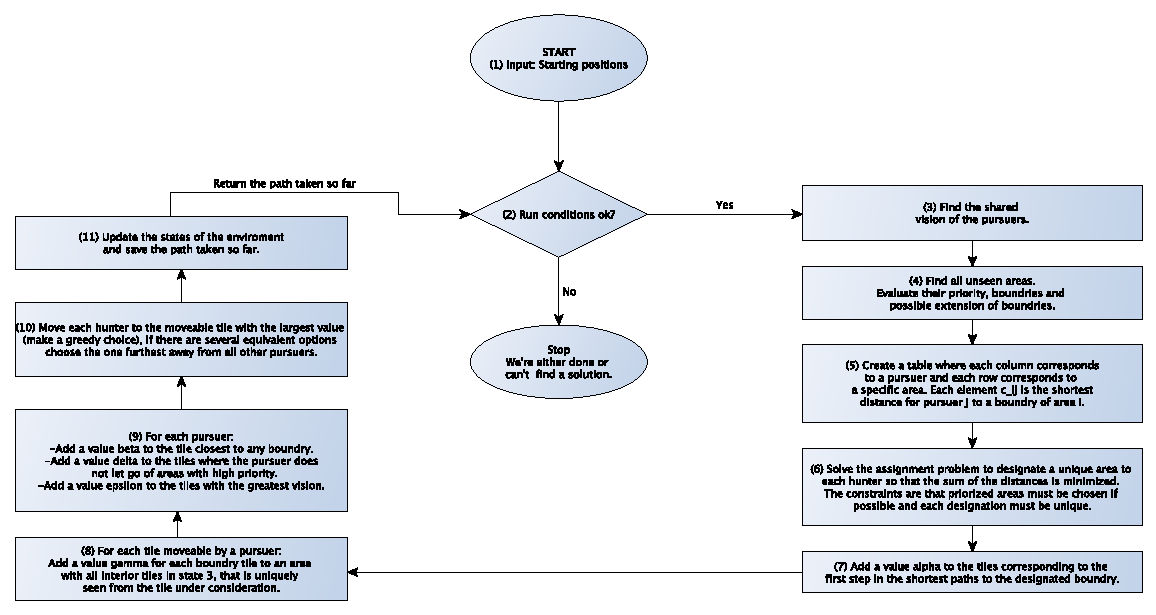
\includegraphics[width=\textwidth]{chapter_4_methods/fittnylle}
  	\caption[Flow chart of greedy algorithm]
  	{Flow chart of greedy algorithm}
	\label{flowchart greedy}
\end{figure}

\begin{enumerate}
\item{} For the first iteration the input is the starting positions of the pursuers. Later when the algorithm is running, the current position of the pursuers will be the input to each iteration.
\item{} At the beginning of each iteration a decision is made whether to make another iteration or not. An iteration should be executed if there exists \emph{tiles} in enviroment that are not \emph{secured} and if the breaking condition is not met. The breaking condition describes the maximum amount of iterations allowed and are given by the main program running the algorithm, so that if no solution can be found the algorithm will abort in due time. 
\item{} Here we find the total field of view of the pursuers team. This will divide the enviroment in seen and unseen \emph{areas}.% as in figure 4.2.(figur som visar geometri f�r omr�den. needed??)   
\item{} All \emph{areas} not visible by the pursuer team are given a priority, a \emph{boundry} and if possible an extended \emph{boundry}. A \emph{boundry} to an \emph{area} is the set of all \emph{tiles} that are both adjacent to some interior \emph{tile} and  also seen by some pursuer. The extended \emph{boundry} to an \emph{area} is the set of all \emph{tiles} such that the whole \emph{area} can be seen from each \emph{tile}. The priority is determined by the geometric properties of the \emph{area} and the \emph{state} of the interior \emph{tiles} of the \emph{area}. If the \emph{area} is \emph{secured} it is only relevant to guard its \emph{boundries}, thus \emph{secured areas }are not to be designated in any of the preceeding steps. Contamined \emph{areas} can be categorised in four different types. In descending order of priority they are:
\begin{itemize} 
\item{}\emph{Areas} with only one \emph{boundry tile}, where the whole \emph{area} can be seen from the \emph{boundry tile}.
\item{}\emph{Areas} with several \emph{boundries tiles}, where the whole \emph{area} can be seen from some \emph{boundry tile}. 
\item{}\emph{Areas} with only one \emph{boundry tile}, but who can not be fully seen from the \emph{boundry}.
\item{}Other \emph{areas}.
\end{itemize} 
\item{} In this step a table of possible choices for the pursuers is created. As mentioned above the \emph{secured areas} should not be a part of the table. The extended \emph{boundries} are to be used when measuring the shortest \emph{path} to a \emph{boundry} for a pursuer. This is because our aim is to \emph{see} the \emph{area}, and the extended \emph{boundries} usually provides shorter \emph{paths} for the pursuers. Each row in the table corresponds to an certain \emph{area} and each column corresponds to a certain pursuer. Every element in the table corresponds to the number of \emph{tiles} in the shortest \emph{path} for the given pursuer to a given \emph{area's boundry} or extended \emph{boundry}. 
\item{} Given the table created we now want to choose as many elements as there are columns, since the columns corresponds to pursuers. The choice is to be made in such a way that there is at most one element chosen from each row and column and so that the sum of the chosen elements is minimized. Also there is a constraint that the rows corresponding to \emph{areas} that can be fully seen from their \emph{boundries} must be chosen if possible. A chosen element $c_{i,j}$ corresponds to designating the \emph{area} of row i to the pursuer of column j. If there are more pursuers than \emph{areas}, an \emph{area} can be designate to more than one pursuer but all \emph{areas} must be designated to at least one pursuer. This step of the algorithm is a special case of the assignment problem and can be solved for instance by the Hungarian method.
\item{} Given the designation made in the previous step, for each pursuer there is at least one \emph{path} of shortest distance to the designated \emph{boundry}. For each pursuer,  add a value $\alpha$ to the \emph{tiles} being the first step of the \emph{paths} with the shortest possible distance to the designated \emph{boundry}.
\item{} By construction each pursuer has at most five feasible \emph{tiles} that it can move to. For each one of these \emph{tiles}, add a value $\gamma$ for every \emph{boundry tile} to a \emph{secured area} that is uniquely seen by this pursuer.
\item{} For each pursuer:
\begin{itemize}
\item{} Add a value $\beta$ the \emph{tile} being closest to any contamined \emph{area}. 
\item{} For every \emph{area} where the whole interior can be seen from its \emph{boundry}. Add a value $\delta$ to all adjacent \emph{tiles} where this \emph{boundry} can be seen.
\item{} Add a value $\epsilon$ to the \emph{tiles} where the pursuers has the largest field of vision.
\end{itemize}
\item{} In the previous steps we have now added at most five values to each \emph{tile} in the proximity of each pursuer. For each pursuer find the \emph{tile} with the largest sum and move the pursuer into this \emph{tile}.
\item{} When the movement is made, update the \emph{states} of the enviroment correspondingly. Save the \emph{path} taken so far. Return the updated \emph{states} and the current positions of the pursuers to the start of the algorithm. 
\end{enumerate}
\subsection{Implementation of the greedy algorithm}
Even though a ready-to-run implementation was not made, many parts of the implementation were finished. In the prefunction all the needed static information about the enviroment is evaluated and saved to a struct. 
\begin{verbatim}
struct Greedy{
int SolutionPath[]; 
struct Node NodeMatrix[][];
int BreakCondition[];
HashTable; 
}
\end{verbatim}
The SolutionPath is an array where index 0 contains the number of pursuers, index 1 contains the iterations made (initially set to zero by the prefunction), and the rest of the indices are the coordinates for each pursuer. The NodeMatrix is the graph created by the simulation enviroment described in Chapter 3. The break condition is simply an integer to describe the maximum allowed iterations. Since the algorithm needs to know the distance and the \emph{path} between two \emph{tiles} and this is saved into a hashtable. To find the shortest \emph{path} and the distance between two tiles the A-star algorithm is used.\\%FIND THE COMPLEXITY OF A-STAR!!! Dijkstra:  algorithm of $O(\vert v \vert^2)$ , a-star is special case of dijkstar? 
%pregreedy:
%a-star to find the distance and the path between any two tiles. describe complexity
%hashtable to access shortest distance in a fast manor, key: (from to)
%descride the greedy struct contents and motivate.
\\The implementation of the algorithm described in the Section 4.2.3 calls for the usage of a couple of interesting algorithms to solve some of the steps. In step four we want to find the interior of all \emph{areas}. This was implemented by first taking any \emph{tile} not part of the pursuers vision. Make a breadth first search to find and mark all the interior \emph{tiles} of this \emph{area}. Find a new unmarked and unseen \emph{tile} and execute another breadth first search. Repeat this until all \emph{tiles} not visible by the pursuer team are marked. The breadth first algorithm's time complexity is $O(\vert V \vert + \vert E \vert)$ \cite{adk8}, where V is the number of vertices in the graph and E is the number of edges.\\
\\For step six in the algorithm (the assignment) the implementation is designed to exaust all possible combinations and then pick the combination giving the smallest sum. The combinations are found by usage of a queue (first in, first out). Here one could try to use the Hungarian method \cite{hungarian} instead, but since the size of the table is usually not very large this algorithm seemed like overkill.  





\section{The Tabu search method approach}
\subsection{Description of Tabu search method}
Tabu search is a metaheuristic \footnote{ metaheuristic: simmular to heuristic with the add on that it solves the problem iterativly} optimization method, designed to search for the global optimum. Meaning that the method, figuratively, has the ability to climb out of a local minimum, and then explore other parts of the domain. There are several methods on how these abilities can be acquired. Tabu search uses a so-called tabu list, intended to make already visited areas in the domain forbidden (``tabu''). Tabu search has a few conseptual buildingblocks and basic ideas, easy to understand but widely varying in difficulty to implement. Consepts which, if well implemented, will give you a highly sofisticated search algorithm. The core buildingblock is, as mentioned before, the tabu list. The ability to render certain regions or moves tabu enables us to create search strategys built on the information at hand, both for a given moment and from prior experiences of the search. Hence tabu search is all about coming up with intelligent rules, that will set a specific move to be tabu or not. Another key buildingblock is the tabu overriding mechanism, in literature named as the aspiration criteria [glover]. Its jobb is to check whether a certain move should be approved even if it initially was set to be tabu. In addition this means that the existence of the aspiration criteria allowes the tabu list to be more strict. (And the search a lot faster.)\\
\\
With these two key buildingblocks one can construct almost any type of logic structure. Which makes the tabu search an highly implementable and adaptive method. A logic structure that can be built upon these two concepts is the actual main idea behind the tabu search method. To understand this concept of tabu search one really needs to get on terms with the random aspects of the algorithm.\\
\\
The tabu list and aspiration criteria only deals with the random selected \textbf{path/moves/solutions}, this means that the current solution is not necessarily a good one. One of the strengths of the tabu search algorithms is that \emph{any solution produced tells something about the problem at hand, independent of the solutions' quality.} What this really means is that a bad solution also yields important information.  Or, to quote Thomas Edison 

\begin{quotation}
\emph{``I have not failed 1,000 times.  I have
successfully discovered 1,000 ways to NOT make a light bulb.''}
\end{quotation}


This insight might seem somewhat basic at first sight, but if implemented in a good way it yields powerful results.\\
\\
In this description certain aspects of the tabu search methods are intentionally neglected. This is in order to make the text more understandable.To gain clairity a generalized tabu search algorithm will described below, in a flow chart and step by step pseudo code.\\
\\
skall laggas in I ordbeskrivnings kappitlet\\
Word convention:\\ 
Complete solution = a set of moves that have solved the problem.\\
Incomplete solution = a set of moves that will not solve the problem.\\
Feasible solution = a set of moves that have not yet solved the problem, or have not yet been evaluated whether it is a complete/incomplete solution.\\
\\

\begin{enumerate}
\item{}Obtiain one or more feasible solutions. These are ususally generated randomly.
\item{}Evaluate the feasible solutions.
\begin{itemize}
\item[-]{}If it's a complete solution, save it. Update tabu list and aspiration criteria accordingly. Go to step five.
\item[-]{}If it's a new best complete solution, save it. Update the tabu list, the aspiration criteria and the stopping criteria accordingly. Go to step five.
\item[-]{}If it's an incomplete solution, maby save it. Update tabu list and aspiration criteria accordingly. Go to step five.
\item[-]{}If still a feasible solution, got to step three.\\
\end{itemize}

\item{}Check it against the tabu list. If not tabu, update tabu list and aspiration criteria accordingly. Go to step five. If tabu, go to step four.
\item{}Check it against the aspiration criteria. \textbf{Override the tabu list. Update tabu list and aspiration criteria accordingly, go to step five. Not override the tabu list, Go to step five}
\item{}Check stopping criteria. If reached, go to step six. If not, go to step one.
\item{}Terminate algorithm, return final solution.
\end {enumerate}



\subsection{Development process of the Tabu search algorithm}
The developement process of the tabu search algorithm will here be formulated and the choices taken along the road expland. One of the features of this project is that it had a strict deadline. This forced the process in a direction so that the ideas needed to be somewhat easy to implement. \\
\\
Let's start by analysing the random generating of moves a.k.a. feasible solution, see step 1 in figur [flowchart]. The first crossroad was encountered when the decission of generating one feasible solution at a time was taken, instead of generating a set of feasible solutions. The reason behind this choice was that the genetic algorithm already had gone down the path of generating a set of feasible solutions \footnote{ refering to poppulation se sechten???}, since diversity was desired.\\
\\The second crossroad, on the subject of generating moves, was whether to generate one move or a series of moves to generate a new feasible solution. 

This decission was harder to make, since both alternatives seemed to yield highly promising but very different algorithms. The implementation of making a series of moves would be an intermediate between the two choices of the first crossroad. And the result would be a receding horizon [referens johan papper] approach where one had to either:
\begin{itemize}
\item[-]{}Produce a large set of series of moves to later sort by fitness, then choose one to check against the tabu list and aspiration critera.
\item[-]{}Generate a single series of moves to check against the tabu list and aspiration critera.
\end{itemize}

Both alternatives would probably have yielded promising algorithms. But the fact that the tabu list and aspiration critera then would have needed abilities of a more analysing type implied that it would be more difficult to implement. This resulted in that this path was scraped. This meant that the one move one feasible solution approach came out ahead.\\
\\
This settled we can now move forward to view the ideas of the tabu list. In the beginning of the development the ideas flourished. Seven different rules where evaluated:
\begin{enumerate}
\item{}For one feasible solution save the past X number of moves for each pursuer and render these moves tabu to be returned to.
\item{}Do not allow moves that results in X number of lost secured areas.
\item{}Make geometricaly based tabus for critical areas:
\subitem{} Regions of corridor like characteristics would not be needed to be walked down if a pursuer saw its end point or if one had a region with an obstacle that one could walk around. Regions with an obstacle of that kind would need two pursuers to be secured, thus it would be tabu to go about and try to secure it alone. And finaly if one hade a tree like corridor system, going about to solve it would only be allowed with the right amount of pursuers.
\item{} Work togheter:
\subitem{} Somewhat similar to tabu rule (3), but with the addon that two pursuers never really need to see each other only share vissible areas. This is  a more general rule that would need to be weighted in the aspriation criteria.
\item{} High valued areas:
\subitem{} Trying to incorporate the idea of getting information even from bad solutions. This would be made by considering the path taken, areas walked upon in a complete solution should be given a value bonus. Or if you look upon it from another angle, areas not walked upon could be set to be tabu. 
\item{} Low valued areas:
\subitem {}An incomplete solution may have a series of moves that have been concentrated on a specific region for to long, hence one could give this areas a value penalty.
\item{} Not alow, or give value penaltys to� moves in already secured areas.
\end{enumerate}

All these tabus needed to be ranked, given a priority level that would be weighted in the aspiration criteria. Also many of the tabu rules listed above needed some sort of worst case senario handeling, to avoid that the algorithm would get stuck.\\
\\This said, let's now diskuss the aspiration critera:
As understood from the text above the aspiration critera needs to incorporate a lot. As a start it needs to have the ability of checking wheter an area is of high or low value. Which then means that the evaluation step in figure [flochart1] needs a fitness calculation function that would depend on the area visited and the shape of the feasible solution. Sad to say this aspiration criteria, would need an overwhelming amount of work to implement. Thus this advanced aspiration criteria was scrapped for a simpler one. This also means that tabu rules (3), (4), (6) and (7) no longer could be implemented. Tabu rule (5) got simplified to:  areas not walked upon where set to be tabu. More about tabu rule (5) later. The more simple aspiration criteria, in the end, only came to be: more of a worst case scenario handling, to avoid the algorithm of getting stuck.\\
\\Tabu rule (5): When this rule first was implemented the idea was that X number of past complete solutions were analysed to check which areas had been walked upon at least once, and render the rest tabu. The problem was however that this wasn't strict enough. So X was set to one. Which in turn led to a new problem. The problem that arouse was that the algorithm now, under certain circumstances, was too hasty in returning a final solution. This was partially solved by a new stoping criteria and ``go about it again criteria''.\\
\\
That was the development process of the tabu search algorithm, the final version can be viewed in figure [ ] and is also discussed in the next section.\\
\subsection{The Tabu search algorithm for our problem}
%kollat hit!
%kollat hit.
%kollat hit.
%kollat hit.
%kollat hit.


The tabu search algorithm used for solving the problem be discussed here.\\
In figur [generella tabu] a generall step by step explanation was made of the tabu search algorithm. In figur [???] a modified version can be seen, intended to illustrate the final algorithm and also to show what functions from to the general algorithm that was removed.\\

\textbf{The following text will be exchanged for a flowchart figure::}\\
1\\
Obtain feasible solution by going one step with each pursuer randomly =>2\\
2\\
Evaluation of the feasible solution\\
If it is a new best complete solution, save it. Update the tabu list, the aspiration criteria and the stopping criteria accordingly. =>5\\
If it is an incomplete solution. Update stopping criteria accordingly. =>5\\
If still a feasible solution => 3\\
3\\
Check it against the tabu list:\\
If not tabu. Update tabu list and aspiration criteria accordingly =>5\\
If tabu => 4\\
4\\
Check it against the aspiration criteria:\\
Override the tabu list. Update tabu list and aspiration criteria accordingly => 5\\
Not override the tabu list=>5\\
5\\
Check stopping criteria\\
If reached = >6 \\
If not =>1\\
6\\
Terminate algorithm, return final solution\\
\textbf{end of flowchart figure}\\

To get a feel for the algorithm and to point out insufficiencys, an explanation of how the algorithm converges is in order.\\
There are two elements in the algorithm that affect the convergens:
\begin{enumerate}
\item{} Tabu roule (5)
\item{} Best-solution-found-so-far stopping criteria. 
\subitem{} Mening that if a solution is found one does not search for a solution with a path of longer length.
\end{enumerate}
To note here is that both convergens helping elements depend on that they actualy hava a complete solution. Meaning that if the algorithm is unlucky in finding the first complete solution, the computational time will rise acordingly. As a said note, this considerable insufficiency migth have been avoided with the more advansed aspiration critera, discussed in section [develupment].

\subsection{Implementation of the Tabu search algorithm}
%In this section certain important aspects of the implementation will be discussed. With the implementation of the tabu search algorithm, a series of parameter values arouse. Parameter values that had three different features: 
%\begin{enumerate}
%\item{} Tabu rule values:
%\subitem{} tabu rule (1)  save_past_X_number_of_moves 
%\subitem{} tabu rule (2)  X_number_of_lost_secured_areas

%\item{} Stopping criteria values:
%\subitem{} 
%\item{} Go agen values:
%\subitem{}
%\end{enumerate}

%Tabu regler värden
%Brytvilkor
%Go agen caracter
%
%#define max_step_minus_in_L_list 20 				
%#define allowed_stat_4_loss 1				
%#define max_antal_INcomplete_tabu_solutions 800
%#define TABU_MAX_LIKA 8
%#define MAX_TABU_STEPS 100	
%#define START_FROM_THE_BEGINING_AGEN_NUMBER 20
%#define to_easy_problem_problem_adjustment_set_nr_steps_to 6
%#define to_easy_problem_problem_adjustment_go_agen_nr 4
%#define Mss_L_fuck_up 5000
%#define Mss_30 30

%Vad ska skrivas hära:
%Punktform:
%•	Random genereringen fesabal solution probelmet köra tills en CompSolution är funnen sen börjar algen AVKLARAD
%•	Parametrarna beskrivning av och varför dessa. 
%•	Tydliga tillkortackommanden inte kunna stå still!!
%•	Beskrivning av K listan
%•	Beskrivning av L listan
%•	Beskrivning av 30 listan





%Skiva ner pretabu
%Tabu 
%Uppdelning etc
%Beskrivning av sättningen av parametrarna List K list 
%Alla konstiga utskrifter grejen
%Hur dom jävla tabuvilkoren hanterades ,ordningen av koden.



\chapter{Results}
The algorithms were run on iMac's with 2.66GHz Intel Core2Duo and 4GB of RAM. Each machine was given environments of a specified size\footnote{Environments of size 5x5, 9x9, 10x10, 15x15 and 20x20 were used}, where the density of obstacles was either 25\% or 40\% of the total area in the environment. Figure \ref{Envs} shows examples of environments of size 10x10 with (a) 25\% obstacle density and (b) 40\% density that were used.\\
\\For the random environment simulations each machine was given 10 randomly generated environments of equal size. Five starting positions were generated, twice for each environment. To decrease the amount of pursuers the starting positions lastly generated were omitted. Each setup of starting positions, number of pursuers and environment was run with the same conditions four times. \\
\\Each algorithm was given a set of parameters that were tuned in order to find a solution with two pursuers, however each environment was run with 5 to 2 pursuers. The algorithms were also given a maximum number of steps allowed for each pursuer to take, set to be long enough to find a solution. The algorithms were then to find a solution of as few steps as possible for a given number of pursuers. If for a given amount of pursuers neither of the algorithms were able to find a solution within the maximum steps allowed, no further attempts of finding a solution with these conditions were made. Neither were any further attempts made for fewer pursuers on these conditions. In table \ref{SimData} the data acquired is summarized.\\
\\For the Manhattan\footnote{A special symmetric environment, see \cite{paper1}} grid the simulation conditions were different. A 5x5 and a 9x9 Manhattan grid was used with 5 to 2 pursuers, starting positions was the upper left corner for all pursuers and cases.\\
%fyll ut med hur!!!
%\\In table \ref{SimData} the "Average step difference" is given by the difference in steps used for the genetic algorithm and tabu search algorithm in successful cases, divided by the number of successful runs for the given environment and number of pursuers. The "Average time" is the time for each run divided by the number of runs, where both successful and unsuccessful runs were counted.
%% Tables with data
In Table \ref{SimData} the ``Average step difference'' describes the difference in \emph{path} length of complete solutions. This value is attained by subtracting the sum of the length of all \emph{complete solutions} of the tabu search algorithm from the sum of the length of all \emph{complete solutions} of the genetic algorithm and divide this by the number of successful runs for the given environment. The ``Average time'' is the time for each run divided by the number of runs, where both successful and unsuccessful runs were counted.
\begin{center}
\begin{table}[t!hb]
\noindent\makebox[\textwidth]{%
\begin{tabular}{| c | r | r | r | r | r | r | r | r | r | r | }
\hline
%%%%%%%%%%%%%%%%%%%%%%%%%%%%%%%%%%%%%%%%%%%%%%%%%%%%%%%%%%%%%%%%%%%%%%
%%                                                                  %%
%%  This is a LaTeX2e table fragment exported from Gnumeric.        %%
%%                                                                  %%
%%%%%%%%%%%%%%%%%%%%%%%%%%%%%%%%%%%%%%%%%%%%%%%%%%%%%%%%%%%%%%%%%%%%%%
Size	&Pursuers	&Runs	&Unsolved	&Unsolved	&Step difference	&Avgerage time	&Average time \\
	&	&	&(Genetic)	&(Tabu)	&(Genetic - tabu)	&Genetic (sec)	&Tabu (sec)\\
\hline
5x5	&5	&80	&0	&0	&0	&0.037	&0.003\\
5x5	&4	&80	&0	&0	&0	&0.049	&0.008\\
5x5	&3	&80	&0	&0	&1	&0.084	&0.010\\
5x5	&2	&80	&0	&0	&0	&0.116	&0.012\\
	&	&	&	&	&	&	&\\
10x10	&5	&96	&0	&0	&228	&45.653	&18.046\\
10x10	&4	&96	&0	&0	&699	&128.613	&44.249\\
10x10	&3	&95	&1	&12	&1397	&312.450	&76.693\\
10x10	&2	&67	&14	&22	&1580	&537.163	&80.843\\
	&	&	&	&	&	&	&\\
15x15	&5	&42	&10	&23	&929	&560.978	&1676.596\\
15x15	&4	&17	&7	&8	&479	&663.767	&1278.498\\
15x15	&3	&3	&3	&3	&0	&1004.250	&459.086\\
	&	&	&	&	&	&	&\\
20x20	&5	&4	&4	&4	&0	&9521.394	&8959.600\\
 
\hline
\end{tabular} }
\caption{Data from simulations.}
\label{SimData}
\end{table}
\end{center}
%% 
%% Environments
\begin{figure}[t!hb]
\begin{center}
\begin{tabular}{| p{0.1cm} | p{0.1cm} | p{0.1cm} | p{0.1cm} | p{0.1cm} | p{0.1cm} | p{0.1cm} | p{0.1cm} | p{0.1cm} | p{0.1cm} | }
\hline
%%%%%%%%%%%%%%%%%%%%%%%%%%%%%%%%%%%%%%%%%%%%%%%%%%%%%%%%%%%%%%%%%%%%%%
%%                                                                  %%
%%  This is a LaTeX2e table fragment exported from Gnumeric.        %%
%%                                                                  %%
%%%%%%%%%%%%%%%%%%%%%%%%%%%%%%%%%%%%%%%%%%%%%%%%%%%%%%%%%%%%%%%%%%%%%%
	&	&0\cellcolor{black}	&	&	&	&	&0\cellcolor{black}	&	&0\cellcolor{black}\\
\hline
	&	&	&	&	&0\cellcolor{black}	&	&	&	&0\cellcolor{black}\\
\hline
0\cellcolor{black}	&0\cellcolor{black}	&	&	&	&	&0\cellcolor{black}	&	&0\cellcolor{black}	&\\
\hline
	&	&	&	&	&0\cellcolor{black}	&	&	&	&\\
\hline
	&	&	&	&	&	&0\cellcolor{black}	&	&0\cellcolor{black}	&0\cellcolor{black}\\
\hline
0\cellcolor{black}	&	&	&	&	&	&	&	&0\cellcolor{black}	&0\cellcolor{black}\\
\hline
0\cellcolor{black}	&0\cellcolor{black}	&	&0\cellcolor{black}	&	&	&	&0\cellcolor{black}	&	&\\
\hline
	&	&	&	&	&0\cellcolor{black}	&	&	&	&\\
\hline
0\cellcolor{black}	&	&	&	&	&	&	&	&	&\\
\hline
	&	&	&	&	&0\cellcolor{black}	&0\cellcolor{black}	&0\cellcolor{black}	&	&\\
 
\hline
\end{tabular}
\hspace{0.5cm}
\begin{tabular}{| p{0.1cm} | p{0.1cm} | p{0.1cm} | p{0.1cm} | p{0.1cm} | p{0.1cm} | p{0.1cm} | p{0.1cm} | p{0.1cm} | p{0.1cm} | }
\hline
%%%%%%%%%%%%%%%%%%%%%%%%%%%%%%%%%%%%%%%%%%%%%%%%%%%%%%%%%%%%%%%%%%%%%%
%%                                                                  %%
%%  This is a LaTeX2e table fragment exported from Gnumeric.        %%
%%                                                                  %%
%%%%%%%%%%%%%%%%%%%%%%%%%%%%%%%%%%%%%%%%%%%%%%%%%%%%%%%%%%%%%%%%%%%%%%
	&	&0\cellcolor{black}	&	&0\cellcolor{black}	&0\cellcolor{black}	&	&0\cellcolor{black}	&	&\\
\hline
	&	&	&	&	&	&	&	&	&0\cellcolor{black}\\
\hline
	&	&	&	&	&0\cellcolor{black}	&	&	&0\cellcolor{black}	&\\
\hline
	&	&	&	&0\cellcolor{black}	&	&	&0\cellcolor{black}	&0\cellcolor{black}	&\\
\hline
	&0\cellcolor{black}	&0\cellcolor{black}	&0\cellcolor{black}	&0\cellcolor{black}	&	&	&0\cellcolor{black}	&0\cellcolor{black}	&\\
\hline
	&	&	&0\cellcolor{black}	&	&	&	&0\cellcolor{black}	&	&\\
\hline
	&	&	&0\cellcolor{black}	&0\cellcolor{black}	&	&	&	&0\cellcolor{black}	&\\
\hline
0\cellcolor{black}	&	&	&	&	&	&	&	&	&\\
\hline
	&	&	&	&	&	&	&	&0\cellcolor{black}	&0\cellcolor{black}\\
\hline
	&	&	&	&	&	&	&	&	&0\cellcolor{black}\\
 
\hline
\end{tabular}
\vspace{0.1cm}\\(a) 10x10 environments with 25\% obstacle density.\\*
\end{center}
\vspace{0.05cm}
\begin{center}
\begin{tabular}{| p{0.1cm} | p{0.1cm} | p{0.1cm} | p{0.1cm} | p{0.1cm} | p{0.1cm} | p{0.1cm} | p{0.1cm} | p{0.1cm} | p{0.1cm} | }
\hline
%%%%%%%%%%%%%%%%%%%%%%%%%%%%%%%%%%%%%%%%%%%%%%%%%%%%%%%%%%%%%%%%%%%%%%
%%                                                                  %%
%%  This is a LaTeX2e table fragment exported from Gnumeric.        %%
%%                                                                  %%
%%%%%%%%%%%%%%%%%%%%%%%%%%%%%%%%%%%%%%%%%%%%%%%%%%%%%%%%%%%%%%%%%%%%%%
0\cellcolor{black}	&	&0\cellcolor{black}	&	&0\cellcolor{black}	&0\cellcolor{black}	&	&	&	&0\cellcolor{black}\\
\hline
	&	&	&	&	&0\cellcolor{black}	&	&	&0\cellcolor{black}	&0\cellcolor{black}\\
\hline
	&0\cellcolor{black}	&	&	&	&	&	&0\cellcolor{black}	&0\cellcolor{black}	&0\cellcolor{black}\\
\hline
0\cellcolor{black}	&0\cellcolor{black}	&0\cellcolor{black}	&0\cellcolor{black}	&	&0\cellcolor{black}	&	&	&0\cellcolor{black}	&0\cellcolor{black}\\
\hline
	&	&	&0\cellcolor{black}	&	&	&	&	&	&0\cellcolor{black}\\
\hline
0\cellcolor{black}	&0\cellcolor{black}	&	&	&	&0\cellcolor{black}	&	&0\cellcolor{black}	&	&0\cellcolor{black}\\
\hline
	&0\cellcolor{black}	&0\cellcolor{black}	&	&0\cellcolor{black}	&0\cellcolor{black}	&	&	&	&\\
\hline
	&0\cellcolor{black}	&	&	&0\cellcolor{black}	&	&0\cellcolor{black}	&	&0\cellcolor{black}	&\\
\hline
	&	&	&0\cellcolor{black}	&0\cellcolor{black}	&	&	&0\cellcolor{black}	&0\cellcolor{black}	&0\cellcolor{black}\\
\hline
	&0\cellcolor{black}	&	&	&	&	&	&	&	&\\
 
\hline
\end{tabular}
\hspace{0.5cm}
\begin{tabular}{| p{0.1cm} | p{0.1cm} | p{0.1cm} | p{0.1cm} | p{0.1cm} | p{0.1cm} | p{0.1cm} | p{0.1cm} | p{0.1cm} | p{0.1cm} | }
\hline
%%%%%%%%%%%%%%%%%%%%%%%%%%%%%%%%%%%%%%%%%%%%%%%%%%%%%%%%%%%%%%%%%%%%%%
%%                                                                  %%
%%  This is a LaTeX2e table fragment exported from Gnumeric.        %%
%%                                                                  %%
%%%%%%%%%%%%%%%%%%%%%%%%%%%%%%%%%%%%%%%%%%%%%%%%%%%%%%%%%%%%%%%%%%%%%%
	&0\cellcolor{black}	&	&0\cellcolor{black}	&0\cellcolor{black}	&0\cellcolor{black}	&0\cellcolor{black}	&	&0\cellcolor{black}	&\\
\hline
	&	&	&	&	&0\cellcolor{black}	&	&	&	&\\
\hline
0\cellcolor{black}	&0\cellcolor{black}	&	&0\cellcolor{black}	&	&0\cellcolor{black}	&0\cellcolor{black}	&	&	&\\
\hline
0\cellcolor{black}	&0\cellcolor{black}	&0\cellcolor{black}	&0\cellcolor{black}	&	&	&0\cellcolor{black}	&	&	&0\cellcolor{black}\\
\hline
0\cellcolor{black}	&	&	&	&	&	&	&	&	&\\
\hline
0\cellcolor{black}	&	&	&	&0\cellcolor{black}	&	&	&	&0\cellcolor{black}	&\\
\hline
0\cellcolor{black}	&	&0\cellcolor{black}	&0\cellcolor{black}	&	&0\cellcolor{black}	&	&0\cellcolor{black}	&	&\\
\hline
0\cellcolor{black}	&	&	&0\cellcolor{black}	&	&0\cellcolor{black}	&0\cellcolor{black}	&	&	&0\cellcolor{black}\\
\hline
	&0\cellcolor{black}	&	&	&	&0\cellcolor{black}	&	&	&	&0\cellcolor{black}\\
\hline
	&	&	&0\cellcolor{black}	&0\cellcolor{black}	&0\cellcolor{black}	&	&0\cellcolor{black}	&	&0\cellcolor{black}\\
 
\hline
\end{tabular}
\vspace{0.1cm}\\(a) 10x10 environments with 40\% obstacle density.\\*
\caption{Examples of environments used}
\end{center}
\label{Envs}
\end{figure}
%% End of environments
%% End of tables
\newpage From the simulations the following observations were made:
\begin{itemize}
\item{For environments of size 15x15 and larger the amount of RAM used was significant.}
\item{The results were dependent on parameter values.}
\item{For environments of size 5x5 were solved with good \emph{quality} for both the tabu search and the genetic algorithm, however tabu search were faster in finding a solution.}
\item{Environments of size 10x10 and larger were not always solved with less than 4 pursuers.}
\item{When tabu search found a solution, it was often of better \emph{quality} than the genetic algorithm.}
\item{For environments of size 10x10 and larger, the genetic algorithm found a solution more often than tabu search.}
\item{For environments of size 10x10 and larger, the \emph{quality} of the solution, if found, varied in steps and computation time.}
\end{itemize}
%%Statistics, tables and a description of the tables. Also motivation to why we have chosen these tables etc.\\\\ %%Results for MILP\footnote{Mixed Integer Linear Programming, see \cite{paper3}} evaluation could also be added here.\\\\

\chapter{Discussion}
This chapter contains analysis of the data collected when running the algorithms and conclusions made during the working process.

\section{The simulation}
The simulation environment developed was usable, but is not without limitations some advantages and disadvantages are listed below.
\begin{itemize}
\item{} As the simulation environment can not merge tiles into one node, something that could be usable for certain geometries such as hallways, the memory usage is proportional to the number of tiles.
\item{} Using a graph means that existing algorithms that are already written for graphs%such as?
can be used, which facilitates implementation. During implementation it is also possible for the nodes to contain a collection information.
\item{} The decision to read environments from files makes the simulation environment usable for many kinds of environments. New environments could easily either be generated or added by hand.
\end{itemize}
%utv�rdera f�rdelar och nackdelar som simuleringsmilj�n besitter.
	%f�rklara visions tillkortakommande
	%kan inte mergea, kr�ver mycker minne
	%graph-approach var bra ide?
	%applicerbar pga filskrivning
\section{Analysis of the simulations}
First off it should be noted that when varying the size of the enviroment certain parameters of the algorithms had to be adjusted. For enviroments of intermediate size a correct adjustment of parameters yielded solutions of significantly higher quality. For larger enviroments it was necessary in order to attain any solution at all. We found no analytical way of adjusting the parameters. A good understanding of the implementation in combination with intuition and testing usually solved the issue. This does not exclude the possibility that there might be a more descisive approach. In fact, based mainly on our intuition, it is most probable.\\
\\As seen in the table \ref{SimData}, given in the previous chapter, for small enviroments both algorithms efficiently provides solutions of high quality, even with a small amount of pursuers. The optimality of the solutions on the randomly generated enviroments is not proven, but it's likely that the provided solutions in most cases are optimal. This assumtion is motivated by the fact that the quality of the solutions rarely differs and the path length is typicaly only a few steps long. It should be noted that the average computational time for these solutions is 3 milliseconds for the tabu search algorithm and 37 milliseconds for the genetic algorithm. These are highly efficient results compared to related work \cite{paper1}.\\%n�mn och j�mf�r manhattan resultat
\\When the size of the enviroment is increased the solutions found are less probable to be optimal. This assumption is motivated by the fact that the quality of the solutions now vary strongly. Also the computational time severely increases with the size of the enviroment. An interesting observation though is to compare how the average computational time for the two algorithms changes as the difficulty increases. The tabu search algorithm is highly efficient if it is able to find a first complete solution. But when running on the bigger areas the average time diverges. On the other hand the genetic algorithm provides reasonable average computational times, and is more reliable to find some solution even for difficult enviroments.\\
\\By combining an indepth understanding of the implementation with the data aquired the following conclusions, and fundamental differences, can be made on the implementation of the algorithms. The tabu algortithm is strongly dependent on finding a complete solution of sufficient quality, in order to be efficient. The reason behind this is that a maximum step length is set dynamicaly by the complete solution found, and tiles not visited in this solution are rendered tabu. Thus, with a complete solution of bad quality there are still a vast amount of aternative paths to consider, which in turn affects the efficency.\\
\\The genetic algorithm does not have the same dependency of finding a complete solution, due to its reproduction properties. This motivates the more robust results on efficency for larger areas, compared to the tabu algorithm. 		
\section{Starting positions}
%l�sningskvalitet starkt beroende av startpositioner.
	%formulera tydligt vilka startf�rh�llanden som avses i problemst�llning hos framtida arbeten.
	%vi har slumpstart, varf�r? vad kan vi se?
	%bed�m kvalitet p� given l�sning utifr�n omst�ndigheter.
	
One of our intentions with this report was to compare 

\section{When do the algorithms fail?}	
%n�r skiter det sig och varf�r?

\section{Future work}
%future work:
	%f�rb�ttra v�rat arbete programmeringsm�ssigt
	%implementera ideer uteblivna pga tidsbrist
		%uteblivna tabuvillkor
		%f�rb�ttra simuleringsmilj�n
		%hybridmetoder
		%implementera greedy, motviera varf�r.
		%om man kunde visa att en optimal l�sning kan formuleras som superposition av dell�sningar skulle algorithmerna kunna �ndras i grunden och bli extremty mycket effektivare.
Improvement on the implementations of the algorithms and the simulation enviroment is probable to give more reliable and promising results. Due to the short amount of time given for a project of this size many short cuts were made intentionally. Another interesting suggestion is to combine the algorithms and create a hybrid method. \\
\\Since the algorithms constructed in this paper are considered to be very efficient for smaller problems it is suggested to investigate whether an global optimal solution could be attained by solving local subproblems.







		

\chapter{Conclusion}
A conclusion of our work, and future work.

\include{FutureWork}
\addcontentsline{toc}{chapter}{References}
\begin{thebibliography}{99}
\selectlanguage{swedish}
 \bibitem{paper1} Johan Thunberg, Xiaoming Hu, Petter "Ogren, A Boolean Control Network Approach to Pursuit Evasion Problems in Polygonial Environments
\bibitem{paper2} Johan Thunberg, Petter "Ogren, A Mixed Integer Linear Programming approach to Pursuit Evasion Problems with optional Connectivity Constraints
\bibitem{paper3} Johan Thunberg, Petter "Ogren, An Iterative Mixed Integer Linear Programming Approach to Pursuit Evasion Problems in Polygonial Environments, 2010 IEEE International Conference on Robotics and Automation

\bibitem{NP} M. R. Garey, D. S. Johnson, Computers and Intractability: A Guide to the Theory of NP-Completeness

 \bibitem{C-bok}Brian W. Kernighan, Dennis M. Ritchie, "The C - Programming Language, (ANSI C Version)", Prentice-Hall of India Pvt. Ltd., New Delhi, 1998
%%%%% Fredrik referenser:
\bibitem{Dumitrescu08} A. Dumitrescu, I. Suzuki and P. Zylinski, Offline variants of the `Lion and Man' problem -- Some problems and techniques for measuring crowdedness and for safe path planning", Theoretical Computer Science, Vol. 399, June 2008, pp. 220-235.
\bibitem{GAHandbook1} Chambers, L.D. PRACTICAL HANDBOOK OF GENETIC ALGORITHMS (GAS) APPLICATIONS, VOL 1, CRC Press 1995, ISBN 0-8493-2519-6.
\bibitem{GAHandbook2} Chambers, L.D. GENETIC ALGORITHMS, VOL 2, CRC Press 1995, ISBN 0-8493-2529-3.
\bibitem{GA-ai} Genetic Algorithms WAREHOUSE, http://geneticalgorithms.ai-depot.com/Tutorial/Overview.html, 2011-05-01
\bibitem{quicksort} Microsoft Support, http://support.microsoft.com/kb/73853, 2011-05-02


%%%%% Felix referenser:
\bibitem{ Glover1}  Glover, F. and Laguna, M. Tabu Search. Dordrecht, Netherlands: Kluwer, 1996.
\bibitem{ Glover2}  Glover, F.; Taillard, E.; and De Werra, D. "A User's Guide to Tabu Search." Ann. Oper. Res. 41, 3-28, 1993.
\bibitem{ Glover3} F. Glover, Tabu search-Part I, ORSA J. Comput. 1(1989)190-206.
\bibitem{ Glover4} F. Glover, Tabu search-Part II, ORSA J. Comput. 2(1990)4-32.
\bibitem{ canada} Michel Gendreau, An Introduction to Tabu Search, Handbook of Metaheuristics 2003, Volume: 57, Publisher: Kluwer Academic Publishers, Pages: 37-54, ISBN: 1402072635, DOI: 10.1007/0-306-48056-5\_2, An Introduction to Tabu Search.

%%%%% Mats referenser:
\bibitem{online lecture} Online lecture, lecture 10 greedy algorithms part one, given by Prof.Sunder Vishwanathan from Department of Computer Science Engineering,IIT Bombay, site: http://nptel.iitm.ac.in/video.php?subjectId=106101060
\bibitem{introduction to Algorithms}Thomas H. Corman, Charles E. Leiserson, Ronald L. Rivest, Clifford Stein, "Introduction to Algorithms", 4th ed. MIT press 2001, chapter 16.
\bibitem{adk8}Lecture notes DD1352, Viggo Kann KTH, http://www.csc.kth.se/utbildning/kth/kurser/DD1352/adk10/schema/ADK-F8.pdf
\bibitem{hungarian}Lecture handouts, Beryl Castello, john hopkins university, http://www.ams.jhu.edu/~castello/362/Handouts/hungarian.pdf
%%%%%
%%%%% Exempel:
%%%%% \bibitem{key} Authors, Title, Publisher, Volume, Publish date, pages.
%%%%% key g�r att det g�r att referera genom \cite{key}, s�tt ett unikt v�rde p� key s� krockar vi inte. F�r d� (exempelvis) [1] i texten, vilket h�nvisar till referens 1.
%%%%%
%%%%%
%%%%%
%%%%%
%%%%%
%%%%% Gamla referenser fr�n exempel-rapporten:
%%%
%%%\bibitem{}Kenneth Hoffmann, Rey Kunze, " Linear Algebra", Prentice-Hall of India Pvt. Ltd., New Delhi, 1997
%%%\bibitem{}G.H. Golub and C. F. Van Loan , " Matrix Computations", Third Edition. The Johns Hopkins University Press, Baltimore, 1996
%%%\bibitem{}David A. Patterson, John L. Hennessy, "Computer Architecture, A Quantitative Approach", Morgan Kaufmann Publications Inc., San Mateo, California, USA, 1990
%%%\bibitem{}Jack Dongarra, Iain Duff, Danny Sorensen, and Henk van der Vorst, Numerical Linear Algebra for High-Performance Computing",Society for Industrial and Applied Mathematics, Philadelphia, 1998
%%%\bibitem{}Abraham Silberschatz, Peter Baer Galvin, "Operating System Concept", Addison Wesley, Reading Massachusetts, USA, 1998 
%%%\bibitem{}John P. Hayes, "Computer Architecture and Organization", McGraw-Hill International Company, Singapore, 1988 
%%%\bibitem{}PVM 3 User Guide and Reference Manual, Edited by Al Gist, Oak Ridge National Laboratory, Engineering Physics and Mathematics Divison, Mathematical Science Section, Oak Ridge, Tennessee, USA, 1991
%%% \bibitem{}PVM's HTTP Site, "http://www.epm.ornl.gov/pvm/"
\selectlanguage{english}
\end{thebibliography}

\appendix{EnvGen.c}
\usepackage{listings}
\lstset{language=C}
\begin{document}
\lstinputlisting{EnvGen.c}
\end{document}
\include{Bilaga2}
\include{Bilaga3}
%%%%%%%%%%%%%%%%%%%%%%


%\bibliography{Reference}
\end{document}
